\section{Реализация инструмента генерации программ}

\subsection{Используемые технологии}

Для разработки инструмента был выбран язык программирования Kotlin \cite{kotlin}. Это язык
программирования, разработанный компанией JetBrains в 2010 году. Основными
преимуществами этого языка программирования являются:
\begin{itemize}
    \item Кроссплатформенность
    \item Возможность интеграции с различными популярными системами сборки
          (Maven, Gradle, etc.)
    \item Возможность интеграции с java без переписывания имеющегося кода
\end{itemize}

Для сборки проекта использована система сборки Gradle \cite{gradle}.

В качестве системы контроля версия используется git, являющийся самой популярной системой
контроля версий на сегодня \cite{git}. Репозиторий с исходным кодом размещен на ресурсе Github
\cite{git} \cite{github} \cite{repo}.


\subsection{Архитектура системы}
Разработанная система имеет клиент-серверную архитектуру с отдельными микросервисами для
некоторых компонент.

Клиентская часть представляет собой веб-сайт с помощью которого пользователь может делать
запросы на получение текста или картинки кода по шаблону (задаче). Также имеется возможность
делать запросы напрямую к API в формате JSON.

Серверная часть состоит из нескольких компонент: непосредственно веб-сервер, система генерации
кода и система проверки ответов студентов. В отдельный микросервис выделена система хранения
текстов и изображений программ, состоящая из базы данных, находящейся в изолированном окружении.

Для автоматизации развертывания системы генерации, поддерживания окружения для хранилища и
системы проверки используются технологии Docker \cite{docker} и docker-compose \cite{docker-compose}.
Благодаря Docker можно создать изолированное окружение (контейнер) для компонента, а docker-compose
позволяет объединять контейнеры в единую локальную сеть.
(\textit{TODO: описать для каких компонентов сделаны контейнеры})

Схема архитектуры показана на изображении \ref{architecture}, ниже подробнее описаны отдельные
компоненты.

\begin{figure}[ht]
    \begin{center}
        \scalebox{0.4}{
            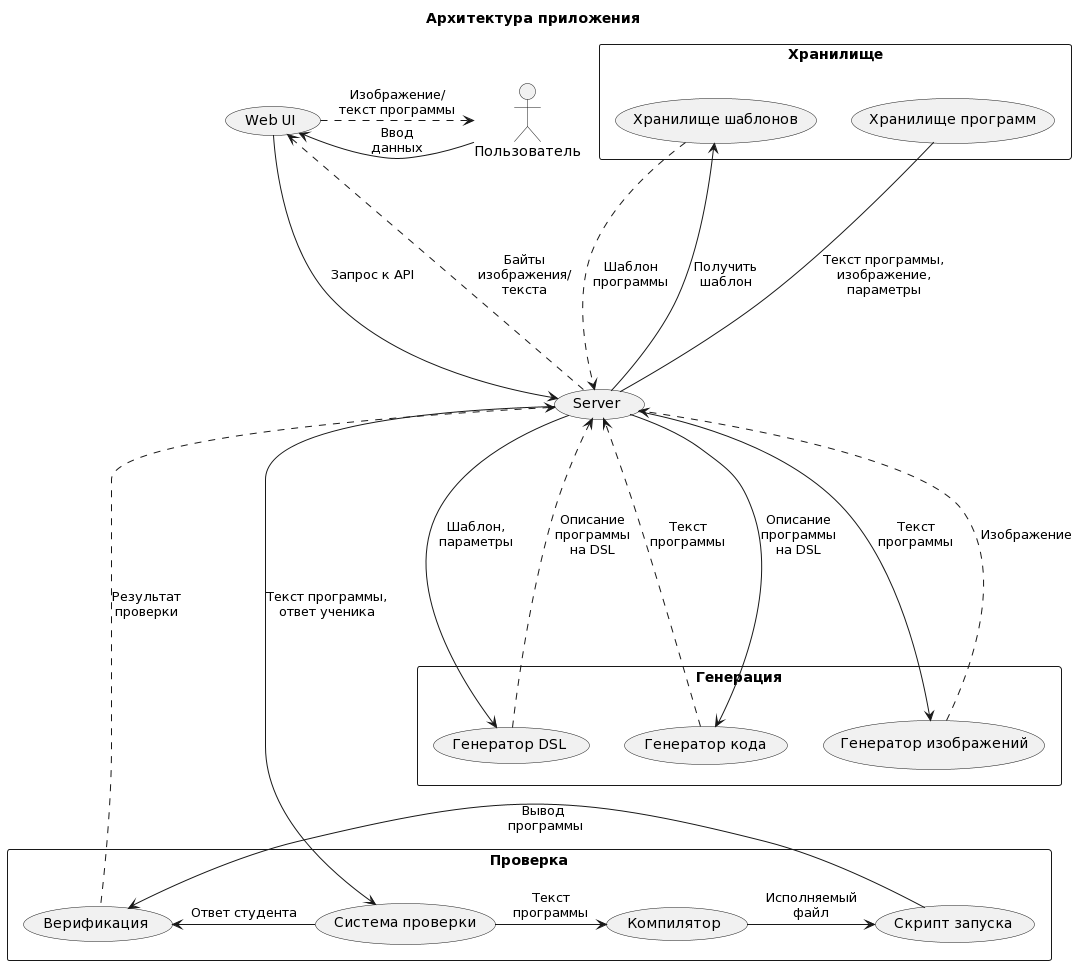
\includegraphics{images/architecture.png}
        }
        \caption{\label{architecture} Архитектура системы генерации программ}
    \end{center}
\end{figure}
\clearpage



\subsection{Компоненты системы}
\subsubsection{Сервер}
Для компонента сервера было принято решение использовать библиотеку Ktor \cite{ktor}, так как
она позволяет быстро создать веб-сервер с нужным функционалом и имеет простой и элегантный API.

(\textit{TODO: описание методов API})

(\textit{TODO: примеры кода})

\subsubsection{Генерация}
Генерация IR (промежуточного представления программы, которое может затем
интерпретироваться в текст на разных языках) работает с помощью подстановки
параметров генерации (атрибутов) и \texttt{seed} для рандомизации в шаблон.

Генерация текста работает с помощью преобразования IR в текст с помощью
специальных классов - code mappers, которые отображают как общие, так и
специфические элементы IR в код. (\textit{TODO: примеры кода})

Генерация изображений реализована с помощью библиотеки \texttt{javax.imageio}
\cite{imageio}. По тексту генерируется изображение в формате jpeg.

\subsubsection{Хранилище сгенерированных программ}
Для поддержки работы с несколькими пользователями необходимо хранить сгенерированные
программы в базе данных. В базе хранятся параметры генерации, которые, вместе с
идентификатором задачи, выступают ключом. Значениями же являются текст и изображение
получившегося кода.

(\textit{TODO: примеры кода})

\subsubsection{Хранилище шаблонов}
Шаблоны задач хранятся в виде файлов на Kotlin, находящихся в отдельном модуле
проекта.
